\chapter{DECORATOR}

Pattern \underline{strutturale} basato su object composition e delegation.

Il suo intento è quello di aggiungere,  dinamicamente, responsabilità ad un oggetto senza influenzare gli altri oggetti. 

Caso d'uso è la GUI dove, per esempio, vogliamo decorare una finestra con un bordo, barra di titolo, barra a scorrimento, ecc\dots

Questo pattern fornisce una soluzione più flessibile riguardo l'utilizzo dell'ereditarietà con la quale si avrebbe un'esplosione di sottoclassi perchè, per cambiare 
una decorazione, dovremmo creare una nuova instanza di un'altra classe.

L'idea di base è quella di racchiudere l'oggetto (\textbf{decorato}) in un altro oggetto (\textbf{decoratore}) che delega i metodi all'oggetto decorato aggiungendo del 
comportamento prima o dopo la delega.

\medskip
\textbf{N.B.}Il decoratore ha la stessa interfaccia dell'oggetto decorato e questo permette di avere tanti decoratori annidati ricorsivamente.

\section{Struttura}

\begin{figure}[H]
    \centering
    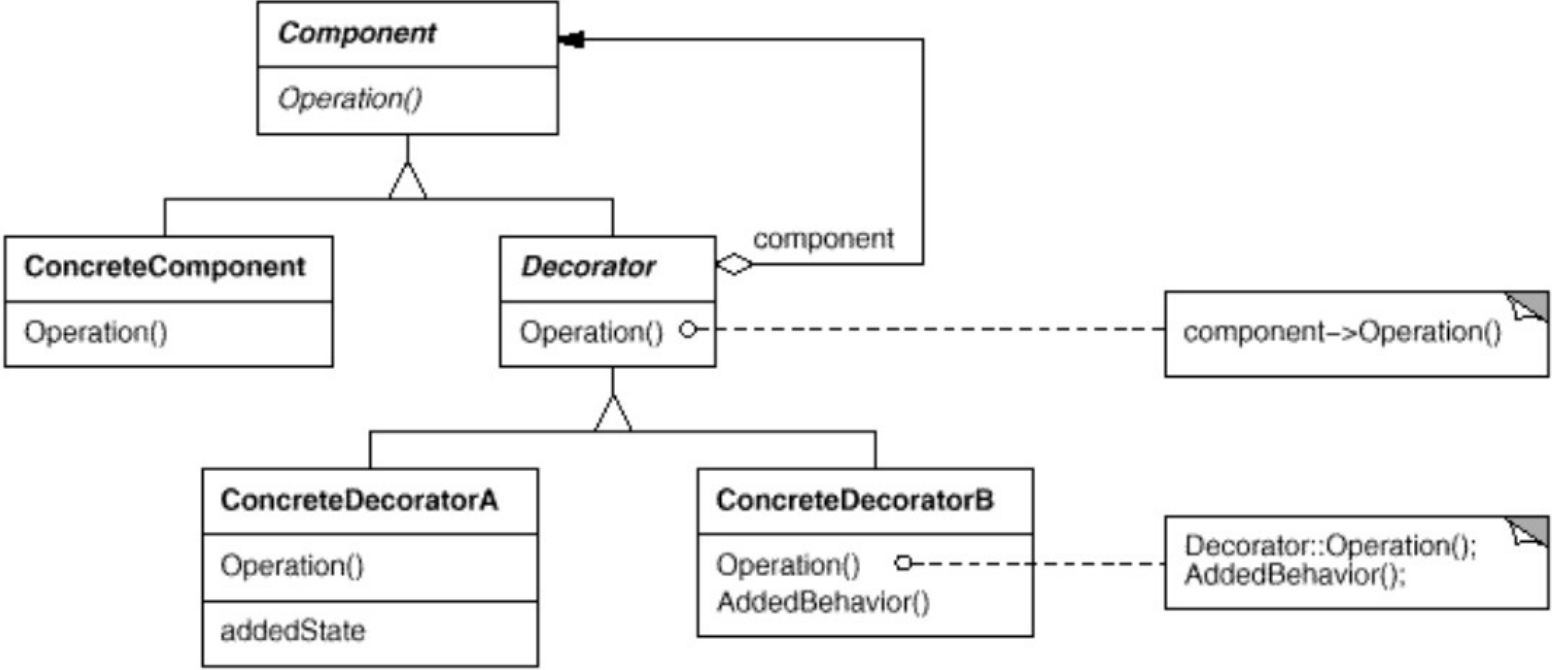
\includegraphics[width=0.5\linewidth]{../../immagini/decorator/struttura_decorator}    
\end{figure}

\textbf{Component} definisce l'interfaccia per gli oggetti a cui è possibile aggiungere, dinamicamente, nuove responsabilità.

\textbf{ConcreteComponent} implementa Component.

\textbf{Decorator} definisce un'interfaccia conforme a Component ed ha un riferimento al Component.

\textbf{ConcreteDecorator} aggiunge responsabilità al Component.
\medskip

Il Decorator inoltra, di default, le richieste al Component e i ConcreteDecorator aggiungono il comportamento prima o dopo l'inoltro.

\medskip
\textbf{N.B.}L'inoltro ci deve sempre essere, altrimenti rompiamo la catena di decorazione.
\medskip

Per l’interface conformance, decorator e componenti devono avere una superclasse comune e tale interfaccia, Component, deve essere il più leggera possibile, deve 
concentrarsi solo sul definire un'interfaccia e non uno stato in quanto mettere troppe funzionalità in Component porterà, le sottoclassi, ad avere funzionalità che 
non gli competono.

\section{Conseguenza}

Un sistema basato su questo pattern avrà a che fare con tanti piccoli oggetti che differiscono per il modo in cui sono iterconnessi e composti.

Questi sistemi sono flessibili e facili da customizzare ma sono difficli da comprendere e debuggare.

Se esiste un solo tipo di decorazione, la classe astratta Decorator non serve.

Uno stesso oggetto Decorator non può essere usato per decorare due componenti.

Potremmo cambiare il componente da decorare se aggiungiamo un setter nel decorator ma lo stesso oggetto decoratore può decorare un solo componente alla volta.

\section{Decorator vs Strategy}

Il Decorator rispetta il principio \textit{"Changing the skin of an object versus changing its guts"} (cambiare la pelle invece delle viscere), cambia la pelle di un 
oggetto avvolgendolo in un decoratore, invece lo Strategy cambia le viscere, ovvero l'oggetto delega allo Strategy il comportamento da seguire.

Component non è a conoscenza dei suoi decoratori, il client utilizza, \textit{senza saperlo}, il Decorator più esterno che farà qualcosa prima o dopo l'inoltro e poi 
dovrà inoltrare al Component che, a sua volta, se sarà un altro decoratore farà la stessa cosa, altrimenti applicherà il comportamento di default.

Nello Strategy, il client \textit{è consapevole} delle diverse implementazioni (ha un riferimento allo Strategy).

Il Decorator ha la stessa interfaccia del suo Component mentre lo Strategy ha la sua interfaccia con diverse implementazioni concrete.

\section{Implementazione senza e con l'entità AbstractDecorator}

Sono due versione del pattern Decorator, nella prima avremo l'interfaccia SaySomething implementata direttamente sia da SaySomethingConcrete che da 
SaySomethingBeforeConcreteDecorator e SaySomethingAfterConcreteDecorator dovee i due decoratori avranno un riferimento a SaySomething e chiameranno direttamente 
l'inoltro su quest'ultimo, aggiungendo del comportamento prima o dopo l'effettivo inoltro.

Nella seconda versione, SaySomething verrà implementata da SaySomethingConcrete e da SaySomethingDecorator che verrà estesa dai decoratori visti prima.

A differenza della prima versione, sarà SaySomethingDecorator ad avere un riferimento a SaySomething e ci chiamerà l'inoltro, mentre i due decoratori si occuperanno di 
aggiungere del comportamento prima o dopo l'inoltro.

I decoratori, non avendo un riferimento diretto a SaySomething, non potranno chiamare l'inoltro su SaySomething, ma lo delegheranno a SaySomethingDecorator attraverso 
il super.

\begin{figure}[H]
\begin{minipage}[c]{9cm}
    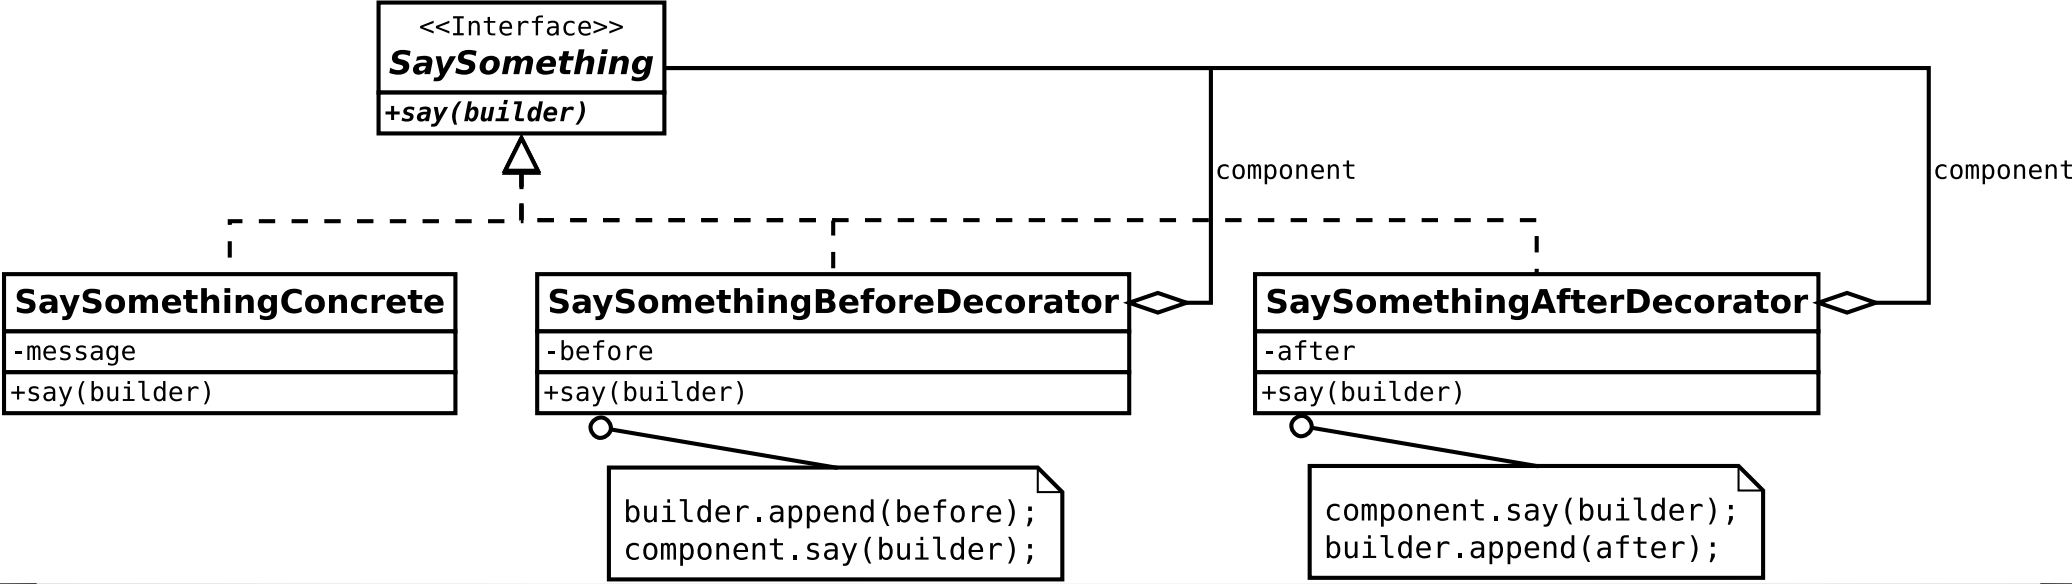
\includegraphics[width=1\linewidth]{../../immagini/decorator/senza_AbstractDecorator}
\end{minipage}
\hfill
\begin{minipage}[c]{8cm}
    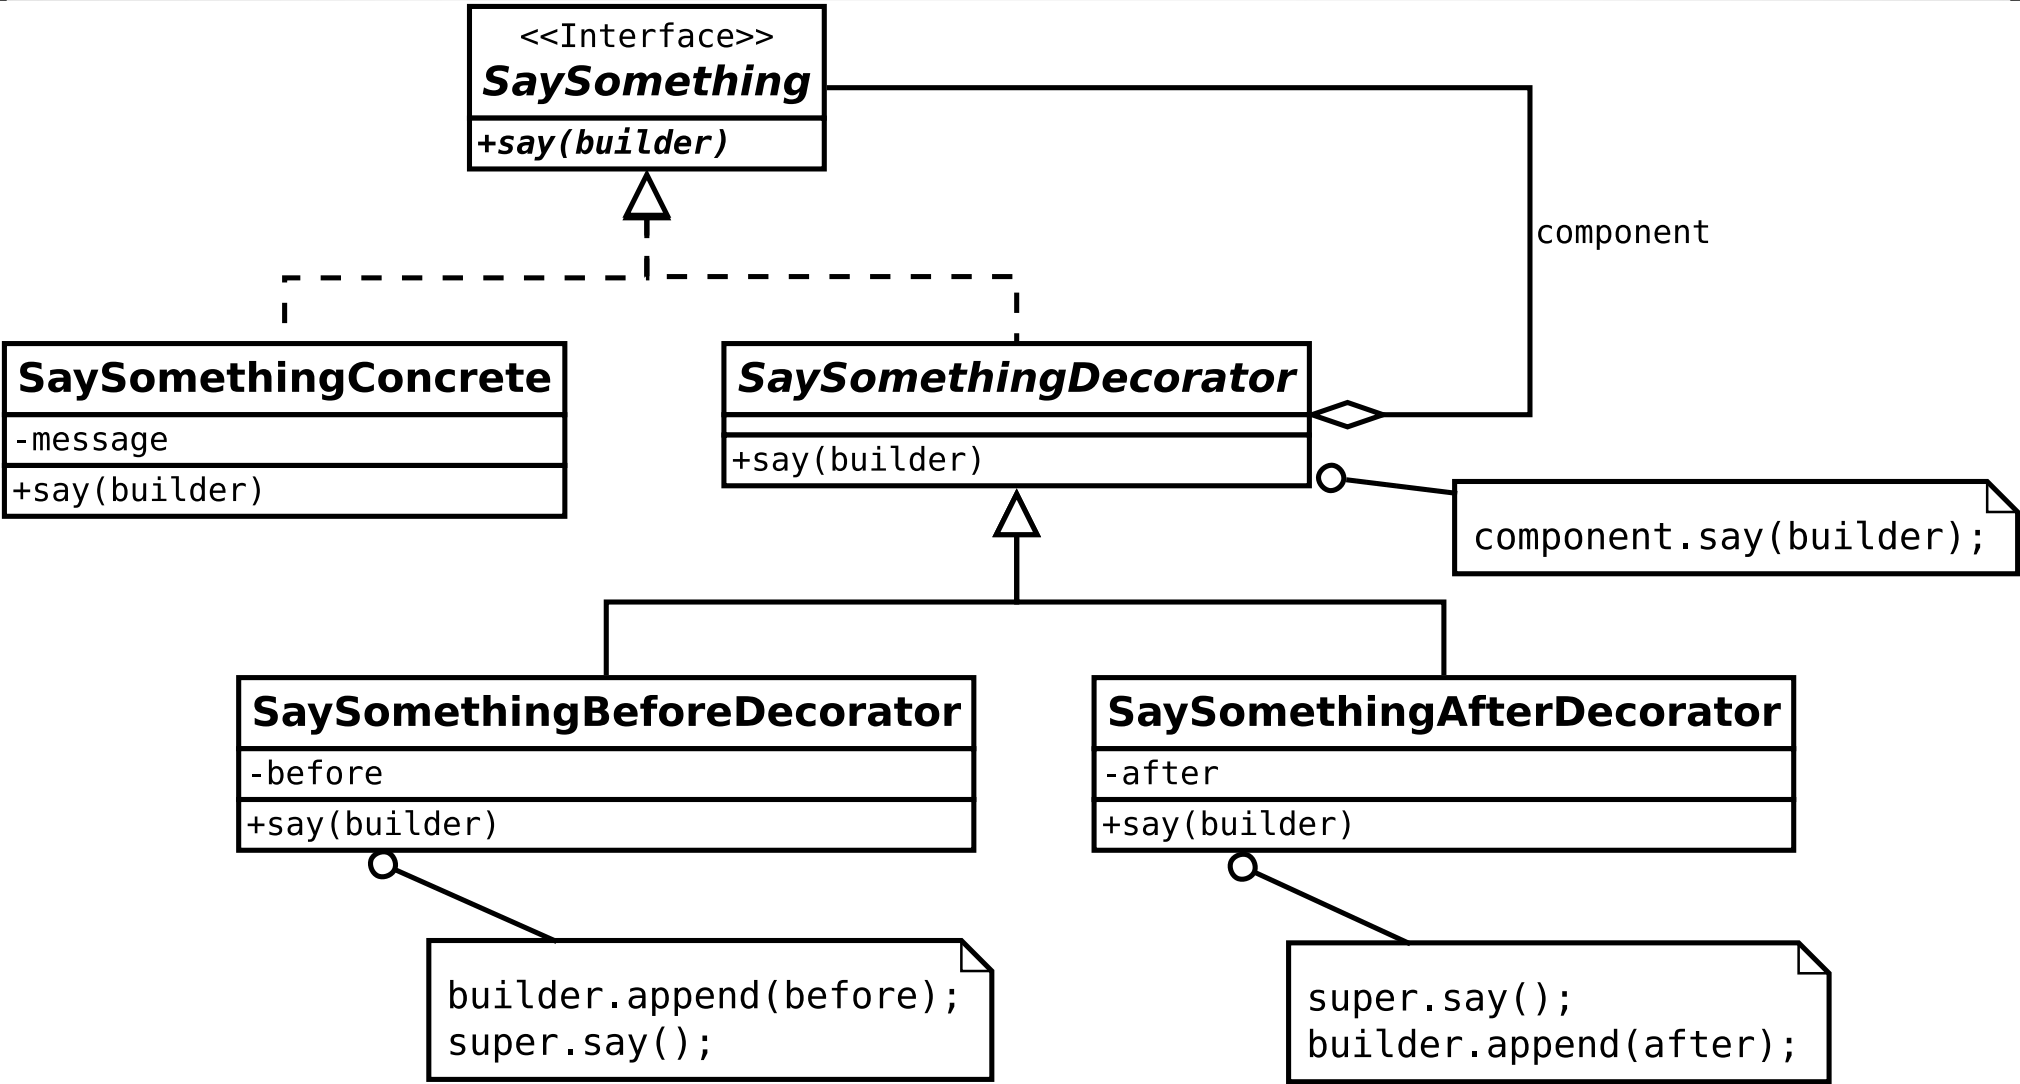
\includegraphics[width=1\linewidth]{../../immagini/decorator/con_AbstractDecorator}
\end{minipage}
\end{figure}

Aggiungere nuovi tipi di decorator è facile, basta implementare/estendere e poi avvolgere SaySomething.

Il difficile è rimuovere un decorator in quanto la catena delle decorazioni deve essere ricreta, dove l'oggetto SaySomething finale non deve essere re-istanziato, 
mentre i decoratori intermedi si.

\medskip
\textbf{N.B.} Quando passiamo il componente da decorare in un decorator, il componente non deve essere null (deve essere documentato nel javadoc), infatti occorre 
fare un controllo la prima volta che ci viene fornito un componente da decorare null (bisognerà anche testare questo scenario).

\section{L'inoltro}

In questo pattern potrebbe capitare di dimenticarsi di inoltrare al Component (non deve succedere).

Per evitare ciò, potremmo rendere il metodo di inoltro, nella classe Decorator, final, e di definire due metodi, astratti, che aggiungono del cambiamento prima e dopo 
l'inoltro.

In questo modo le sottoclassi non potranno dimenticarsi di inoltrare al componente, anche perchè non possono ridefinirlo essendo final, ma avranno il compito di 
implementare i metodi astratti definiti in Decorator.

Il fatto rendere il metodo final e lasciare alcuni suoi passi astratti è un esempio di template method, molti pattern sono usati insieme.

\section{Lambda}

Il pattern Decorator sfrutta il meccanismo dell'ereditarietà, object composition e delegation per sopperire alla mancanza della composizione di funzioni.

Se il linguaggio supporta le lambda, allora, invece di usare i tre meccanismi, possiamo usarle per avere lo stesso risultato ma, a quel punto, non parliamo più di 
Decorator.

Le lambda si usano con le interfacce funzionali (un solo metodo), quindi è applicabile solo al Component che ha uno ed un solo metodo da decorare.

Quindi, nell'esempio visto prima, SaySomething è un'interfaccia funzionale, quindi eleggibile all'utilizzo delle lambda.

Una stessa lambda può essere usata più volte all'interno di una composizione (invece con i decorator dovevamo creare obbligatoriamente due instanze per la stessa 
funzione), inoltre la composizione di una lambda è \textit{lineare} (fluent interface), mentre la composizione del Decorator è \textit{annidata} (la linearità è 
più leggibile).